\section{Results}
\label{sec:results}

This section presents the results and data obtained from the evaluations and compares them with each other.

\begin{figure}[htbp]
  \centering
  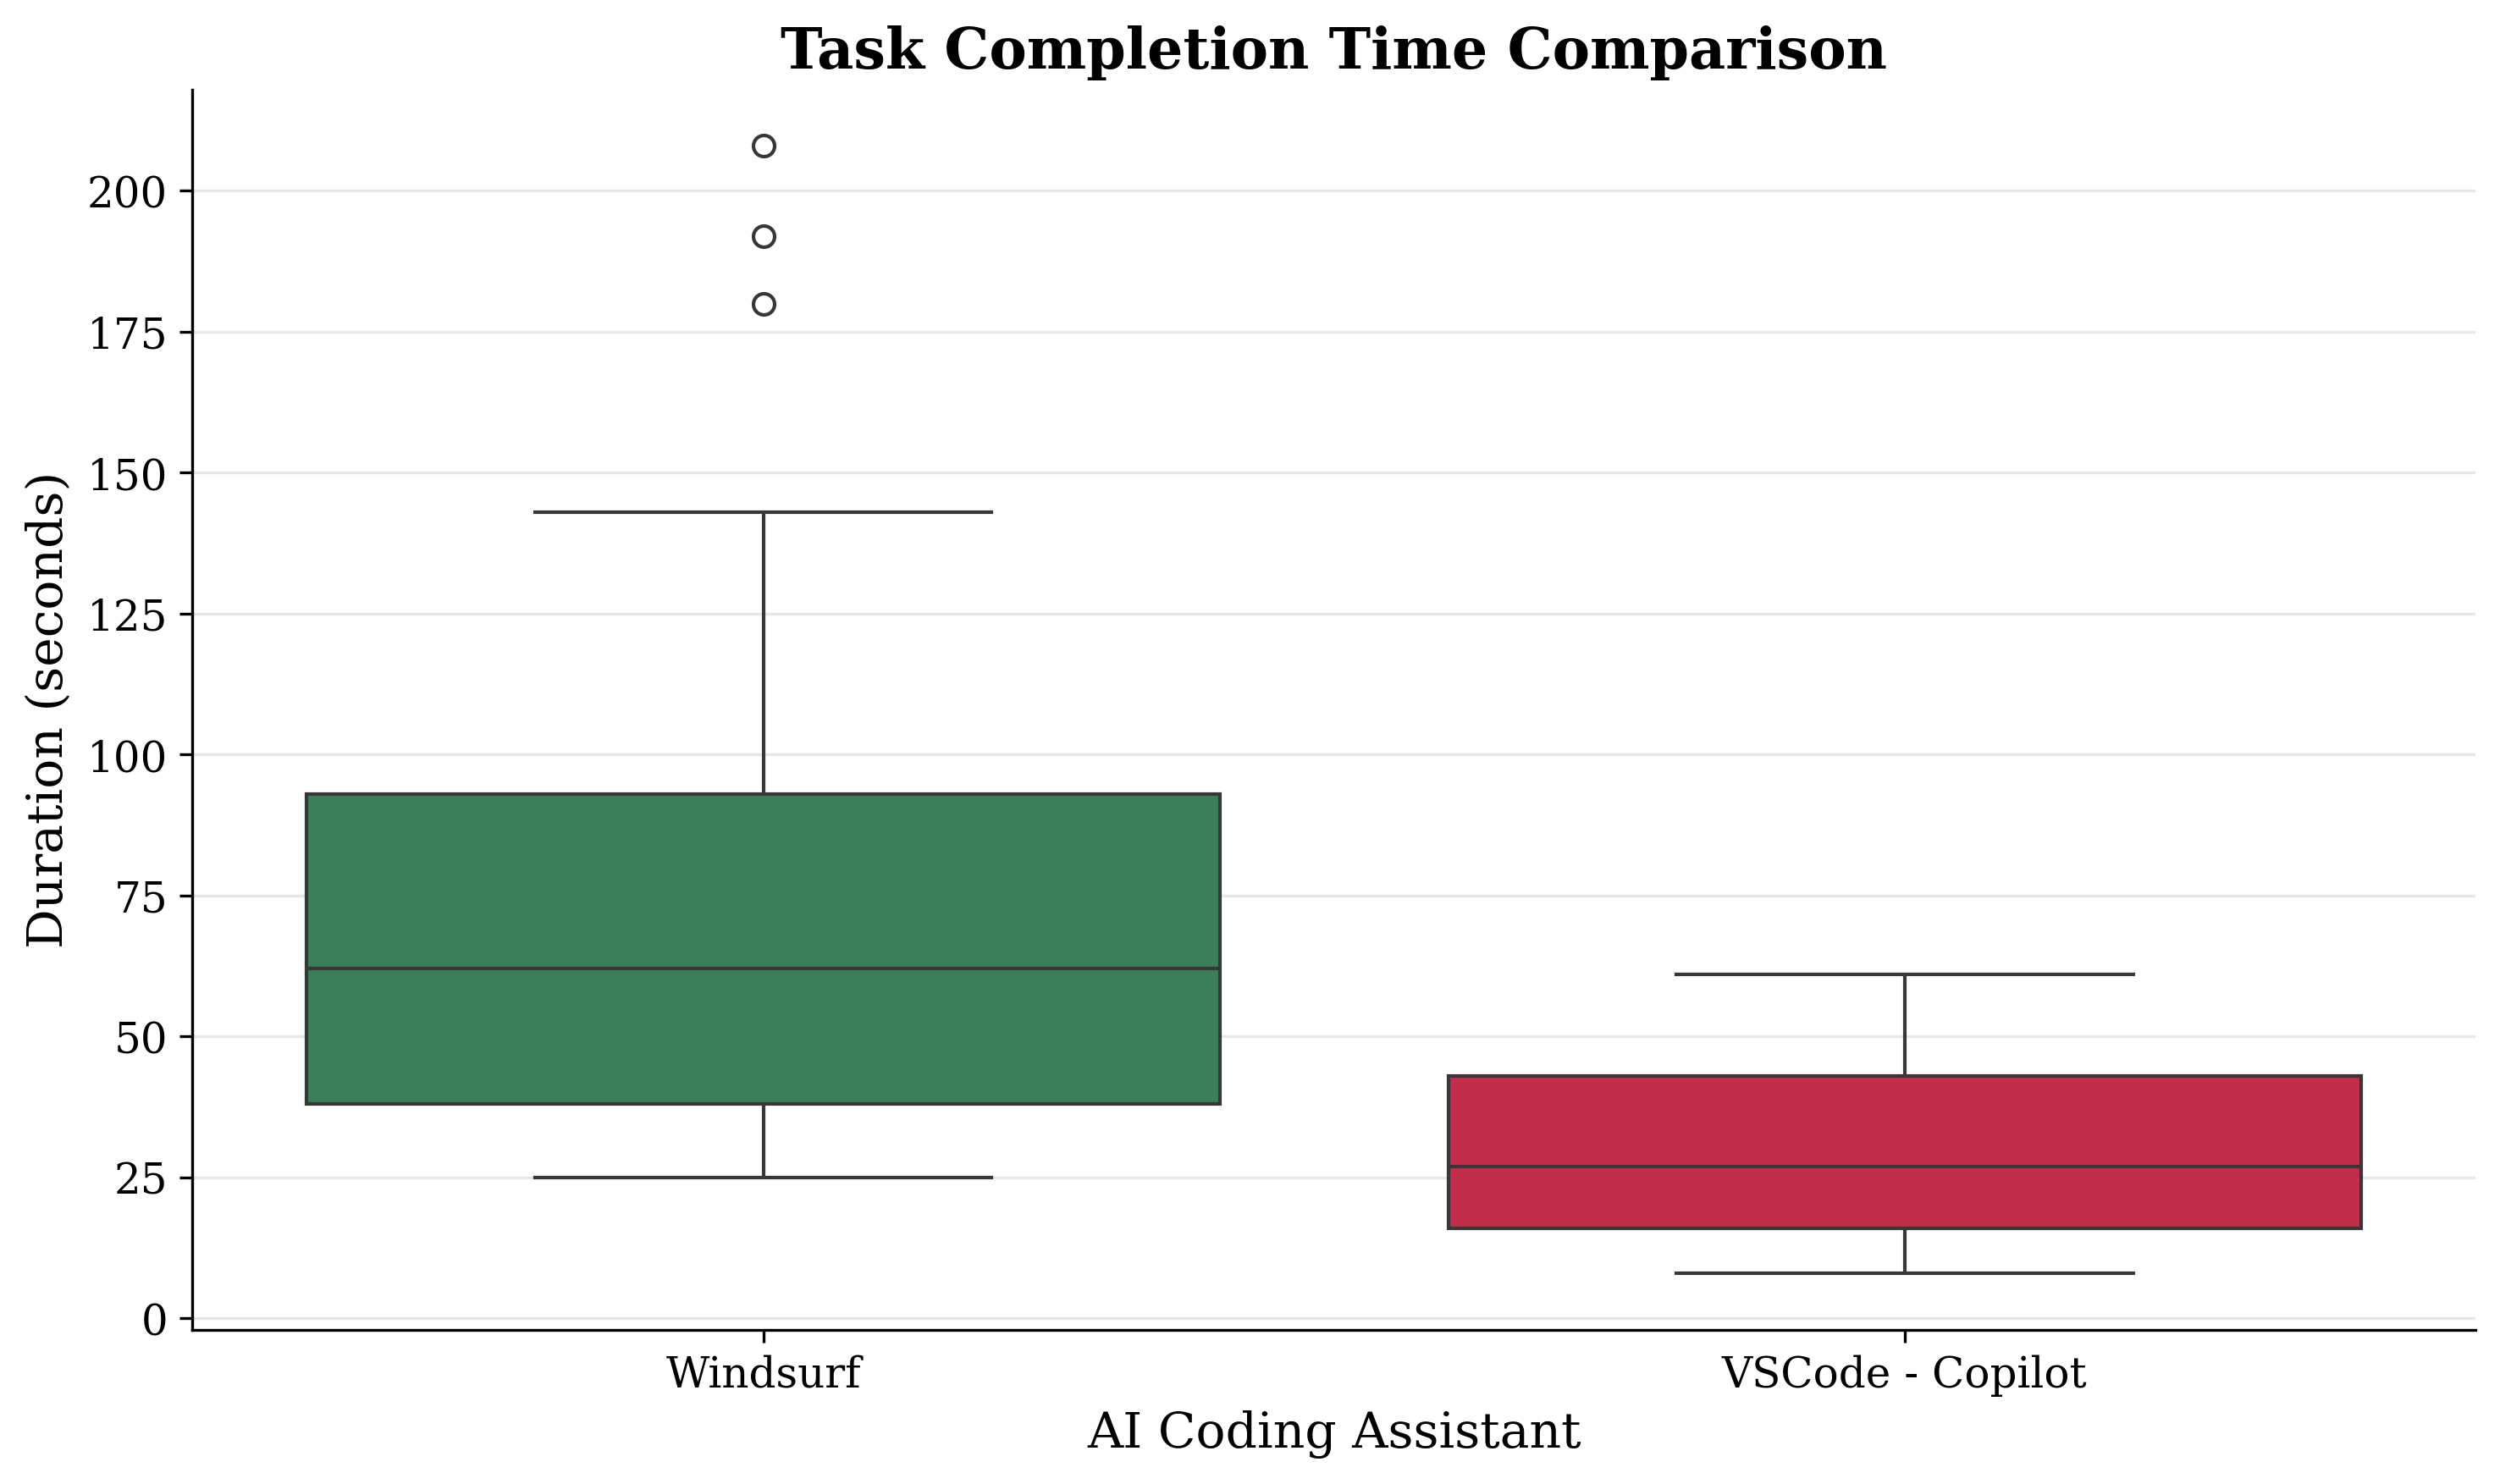
\includegraphics[width=1\linewidth]{images/4_duration_comparison.png}
  \caption{Compared the execution speed across all executions of Windsurf Cascade and Github Copilot}
  \label{fig:runtime-comparison}
\end{figure}


Figure \ref{fig:runtime-comparison} shows a comparison of the average execution speed and distribution of the systems across all executed prompts and iterations. Windsurf Cascade achieved an average speed of 75.1 seconds, while Github Copilot via VSCode achieved an average execution speed of 29.2 seconds. Github Copilot remains very consistent across all executions, while Windsurf Cascade achieved large fluctuations in execution speed. The longest execution time achieved by Windsurf was 208 seconds for the prompt ''C1'' in run two.

\begin{figure}[htbp]
  \centering
  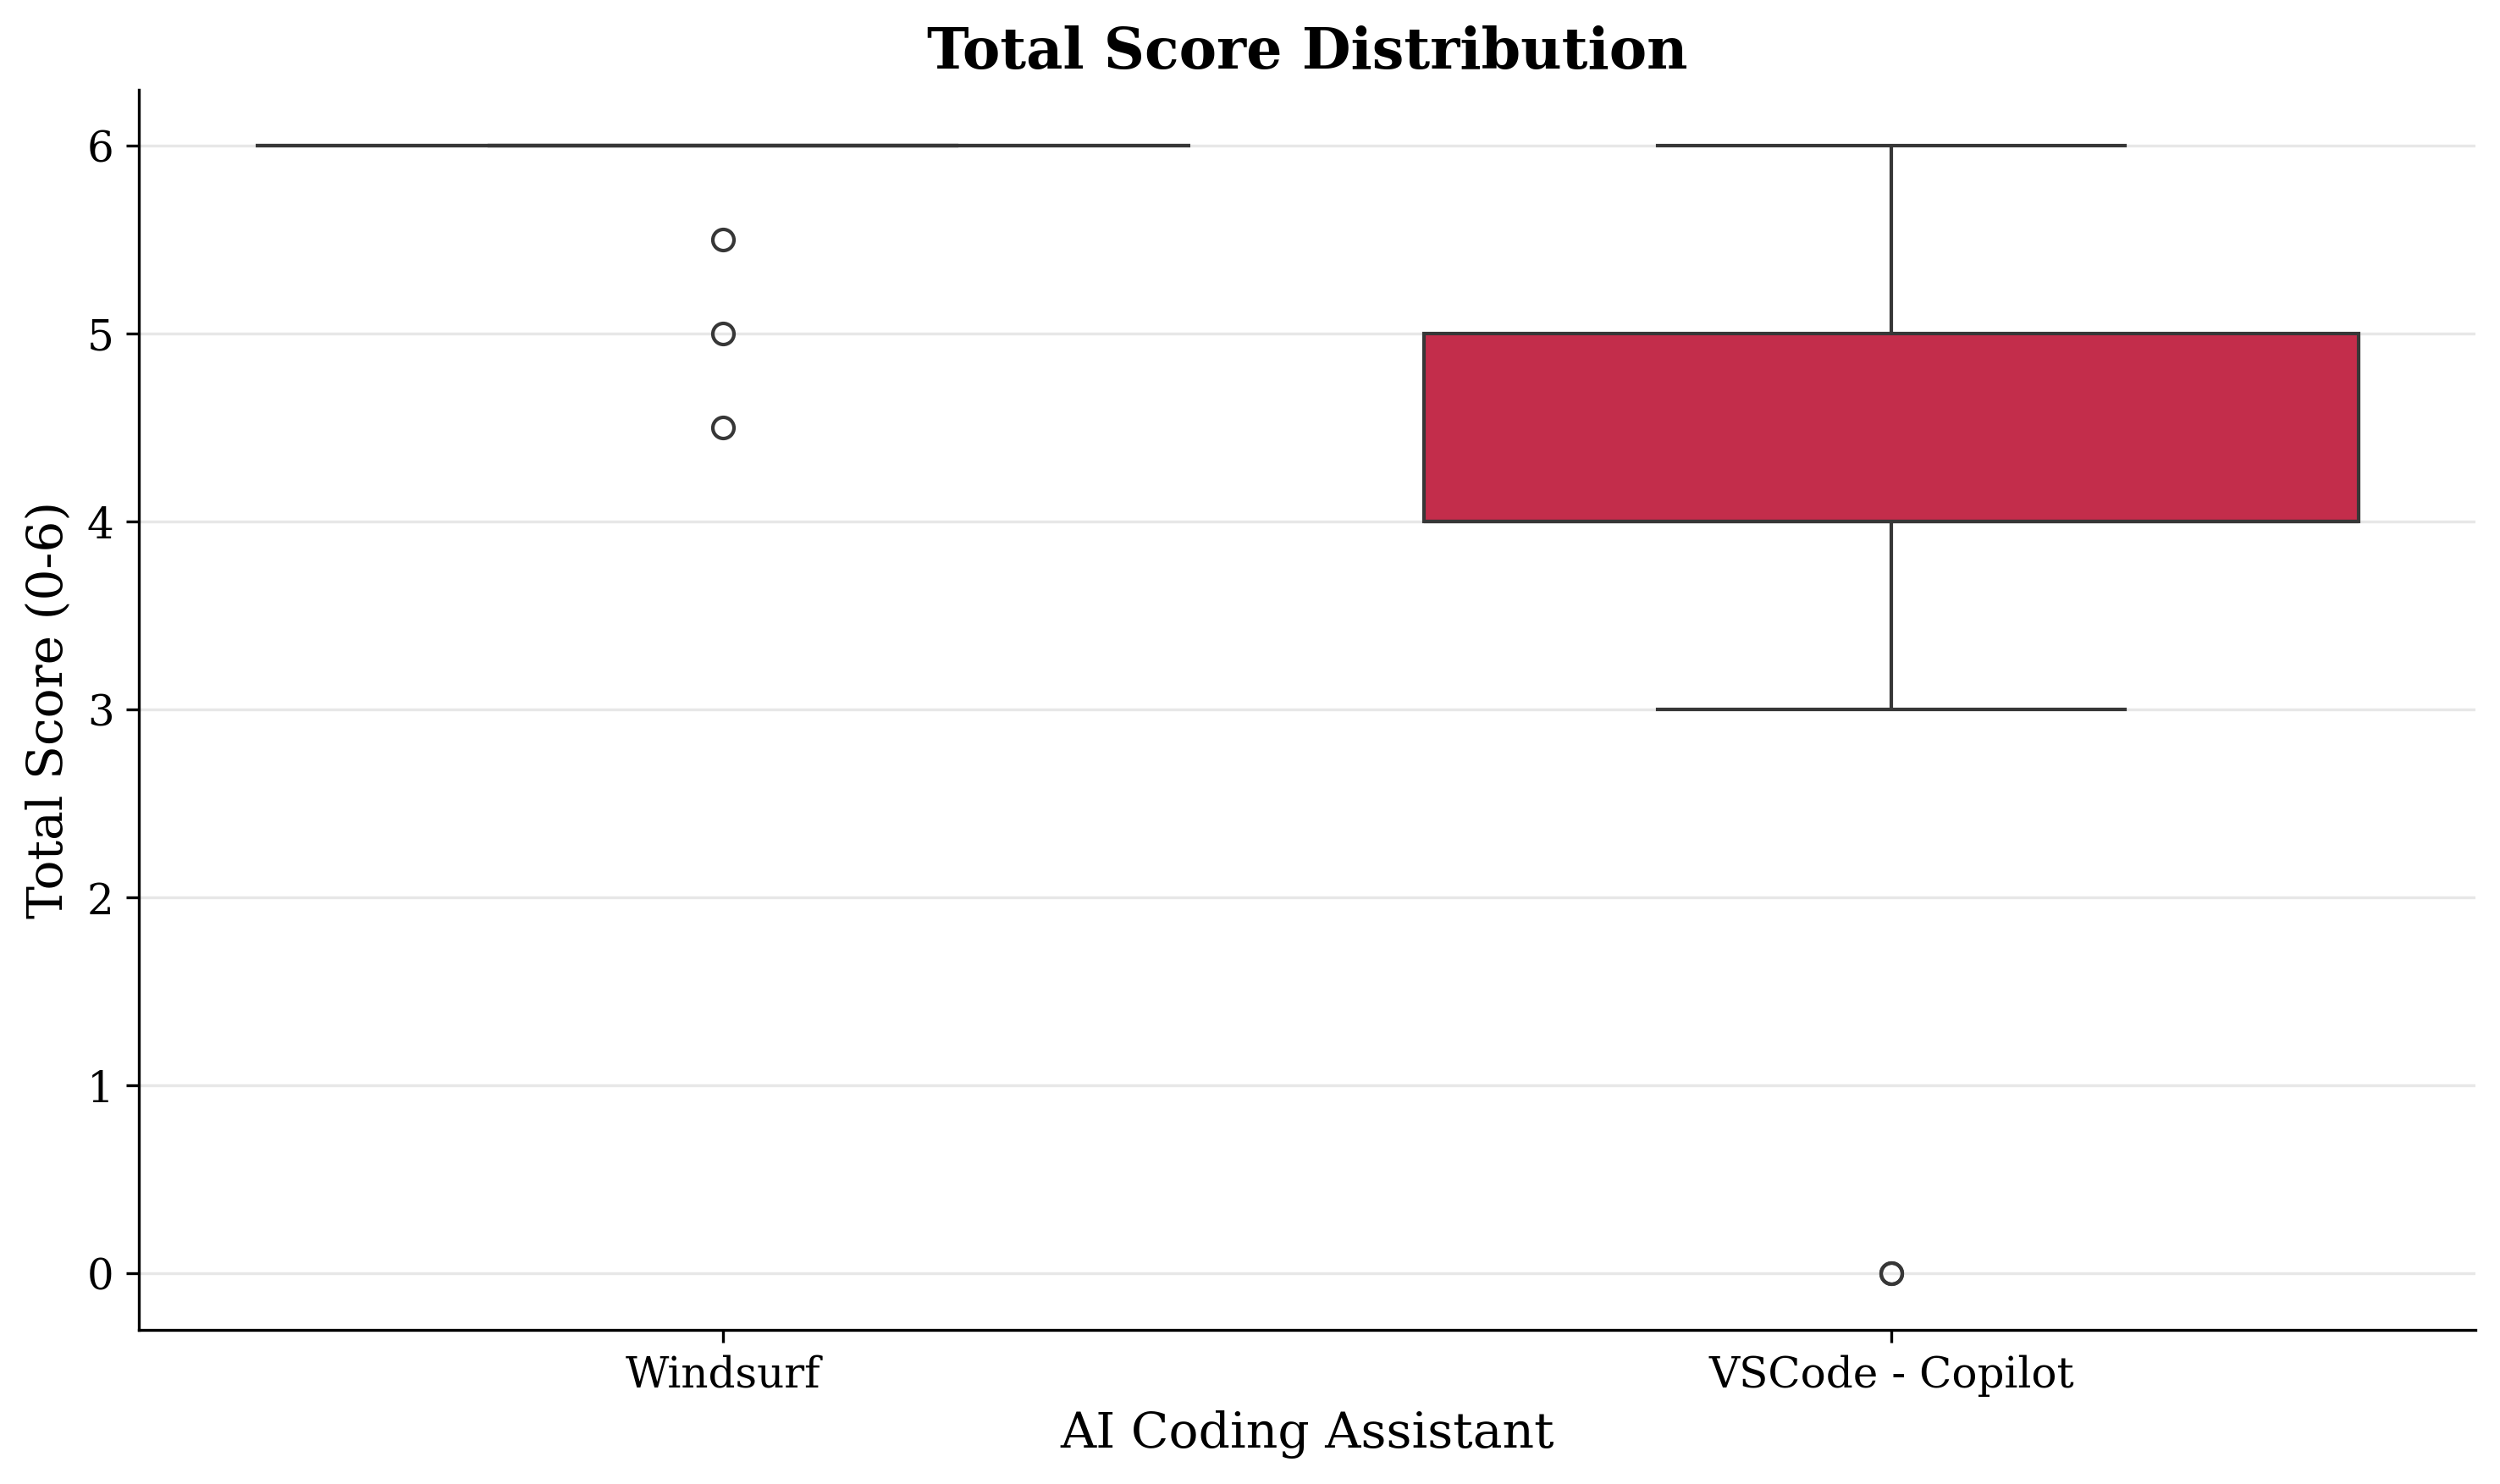
\includegraphics[width=1\linewidth]{images/2_score_distribution.png}
  \caption{Compared the total score distribution across all executions of Windsurf Cascade and Github Copilot}
  \label{fig:score-distribution}
\end{figure}


Figure \ref{fig:score-distribution} shows the average distribution of points for each system across all tasks and runs. Windsurf Cascade achieved an average score of 5.91 points with a standard deviation $\sigma$ of 0.32 points. Github Copilot achieved an average score of 4.06 points with a standard deviation $\sigma$ of 1.35 points. 


\begin{figure}[htbp]
  \centering
  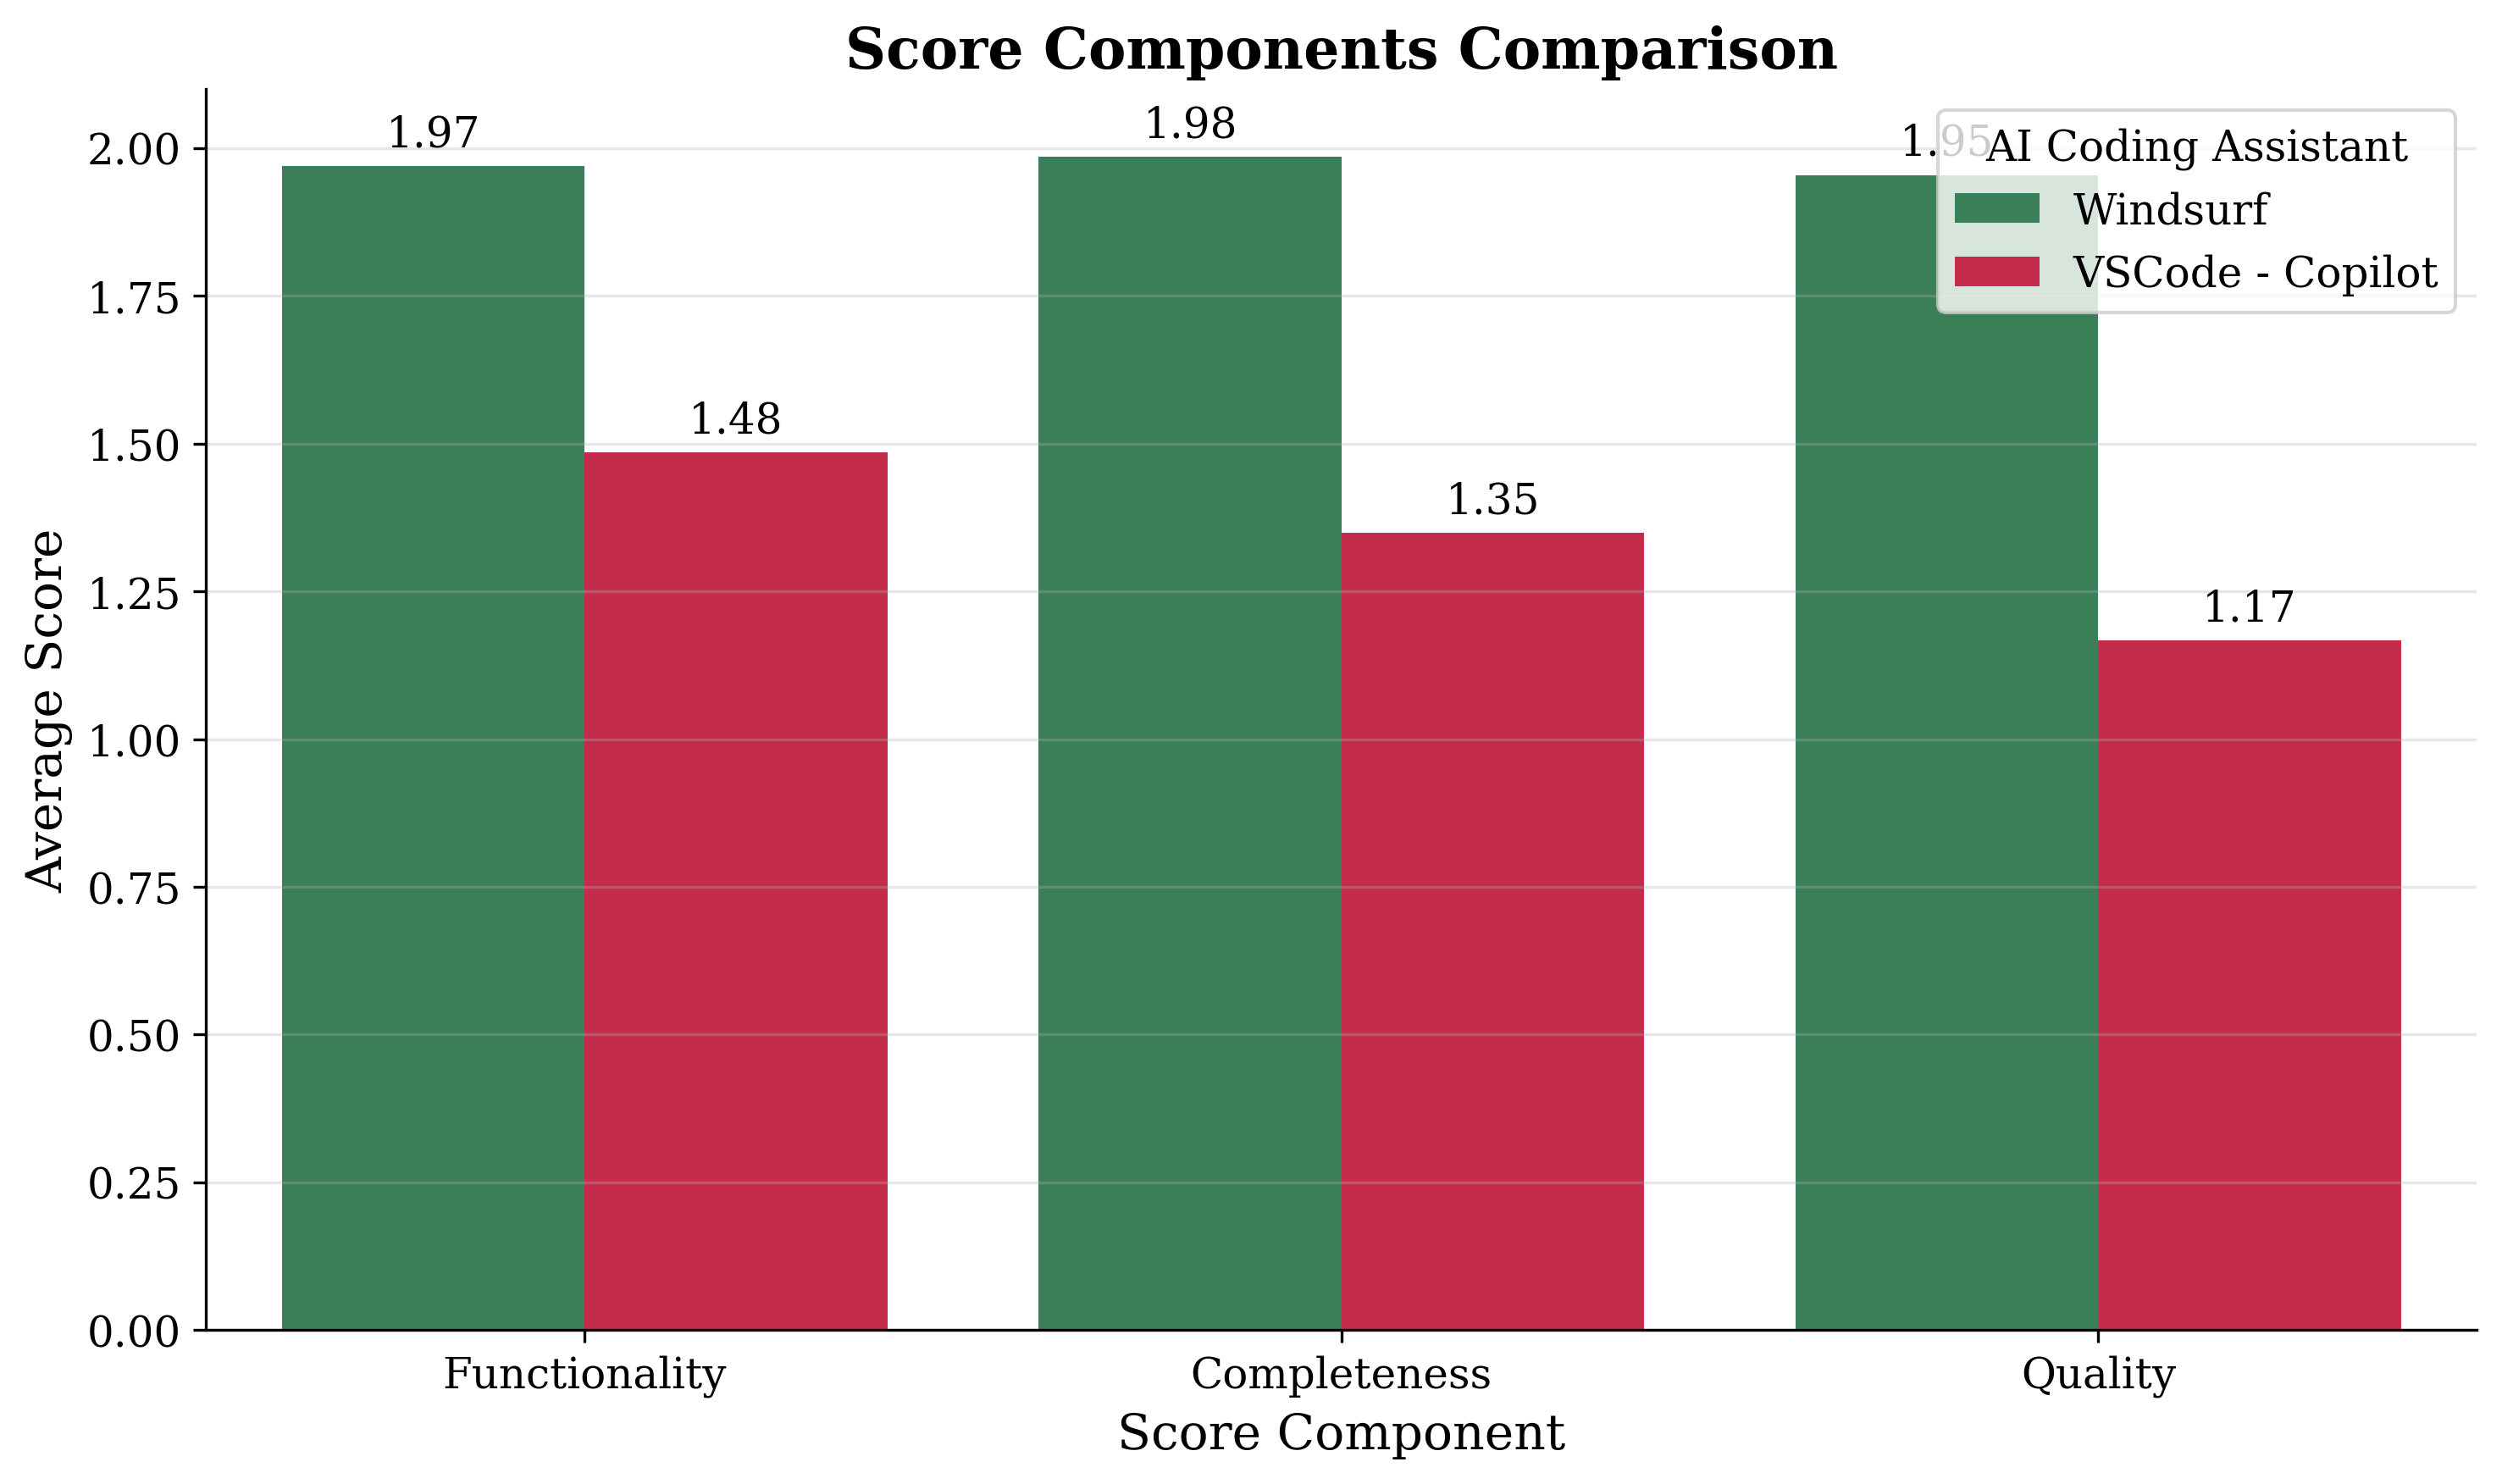
\includegraphics[width=1\linewidth]{images/5_score_components.png}
  \caption{Compared the score components of all executions of Windsurf Cascade and Github Copilot}
  \label{fig:score-components}
\end{figure}

Figure \ref{fig:score-components} shows a comparison of Windsurf Cascade and Github Copilot via VSCode according to the three evaluation criteria or components of the evaluation. The graph shows the average scores of the respective systems across all runs based on the criteria of quality, functionality and completeness. Windsurf Cascade achieved an average score of 1.97 out of 2 points for functionality. Windsurf Cascade achieved an average score of 1.98 out of 2 points for completeness and an average score of 1.95 out of 2 points for quality. Github Copilot via VSCode, on the other hand, achieved an average score of 1.48 out of 2 points for functionality, an average score of 1.35 points for completeness and a score of 1.17 out of 2 points for quality.


\begin{figure}[htbp]
  \centering
  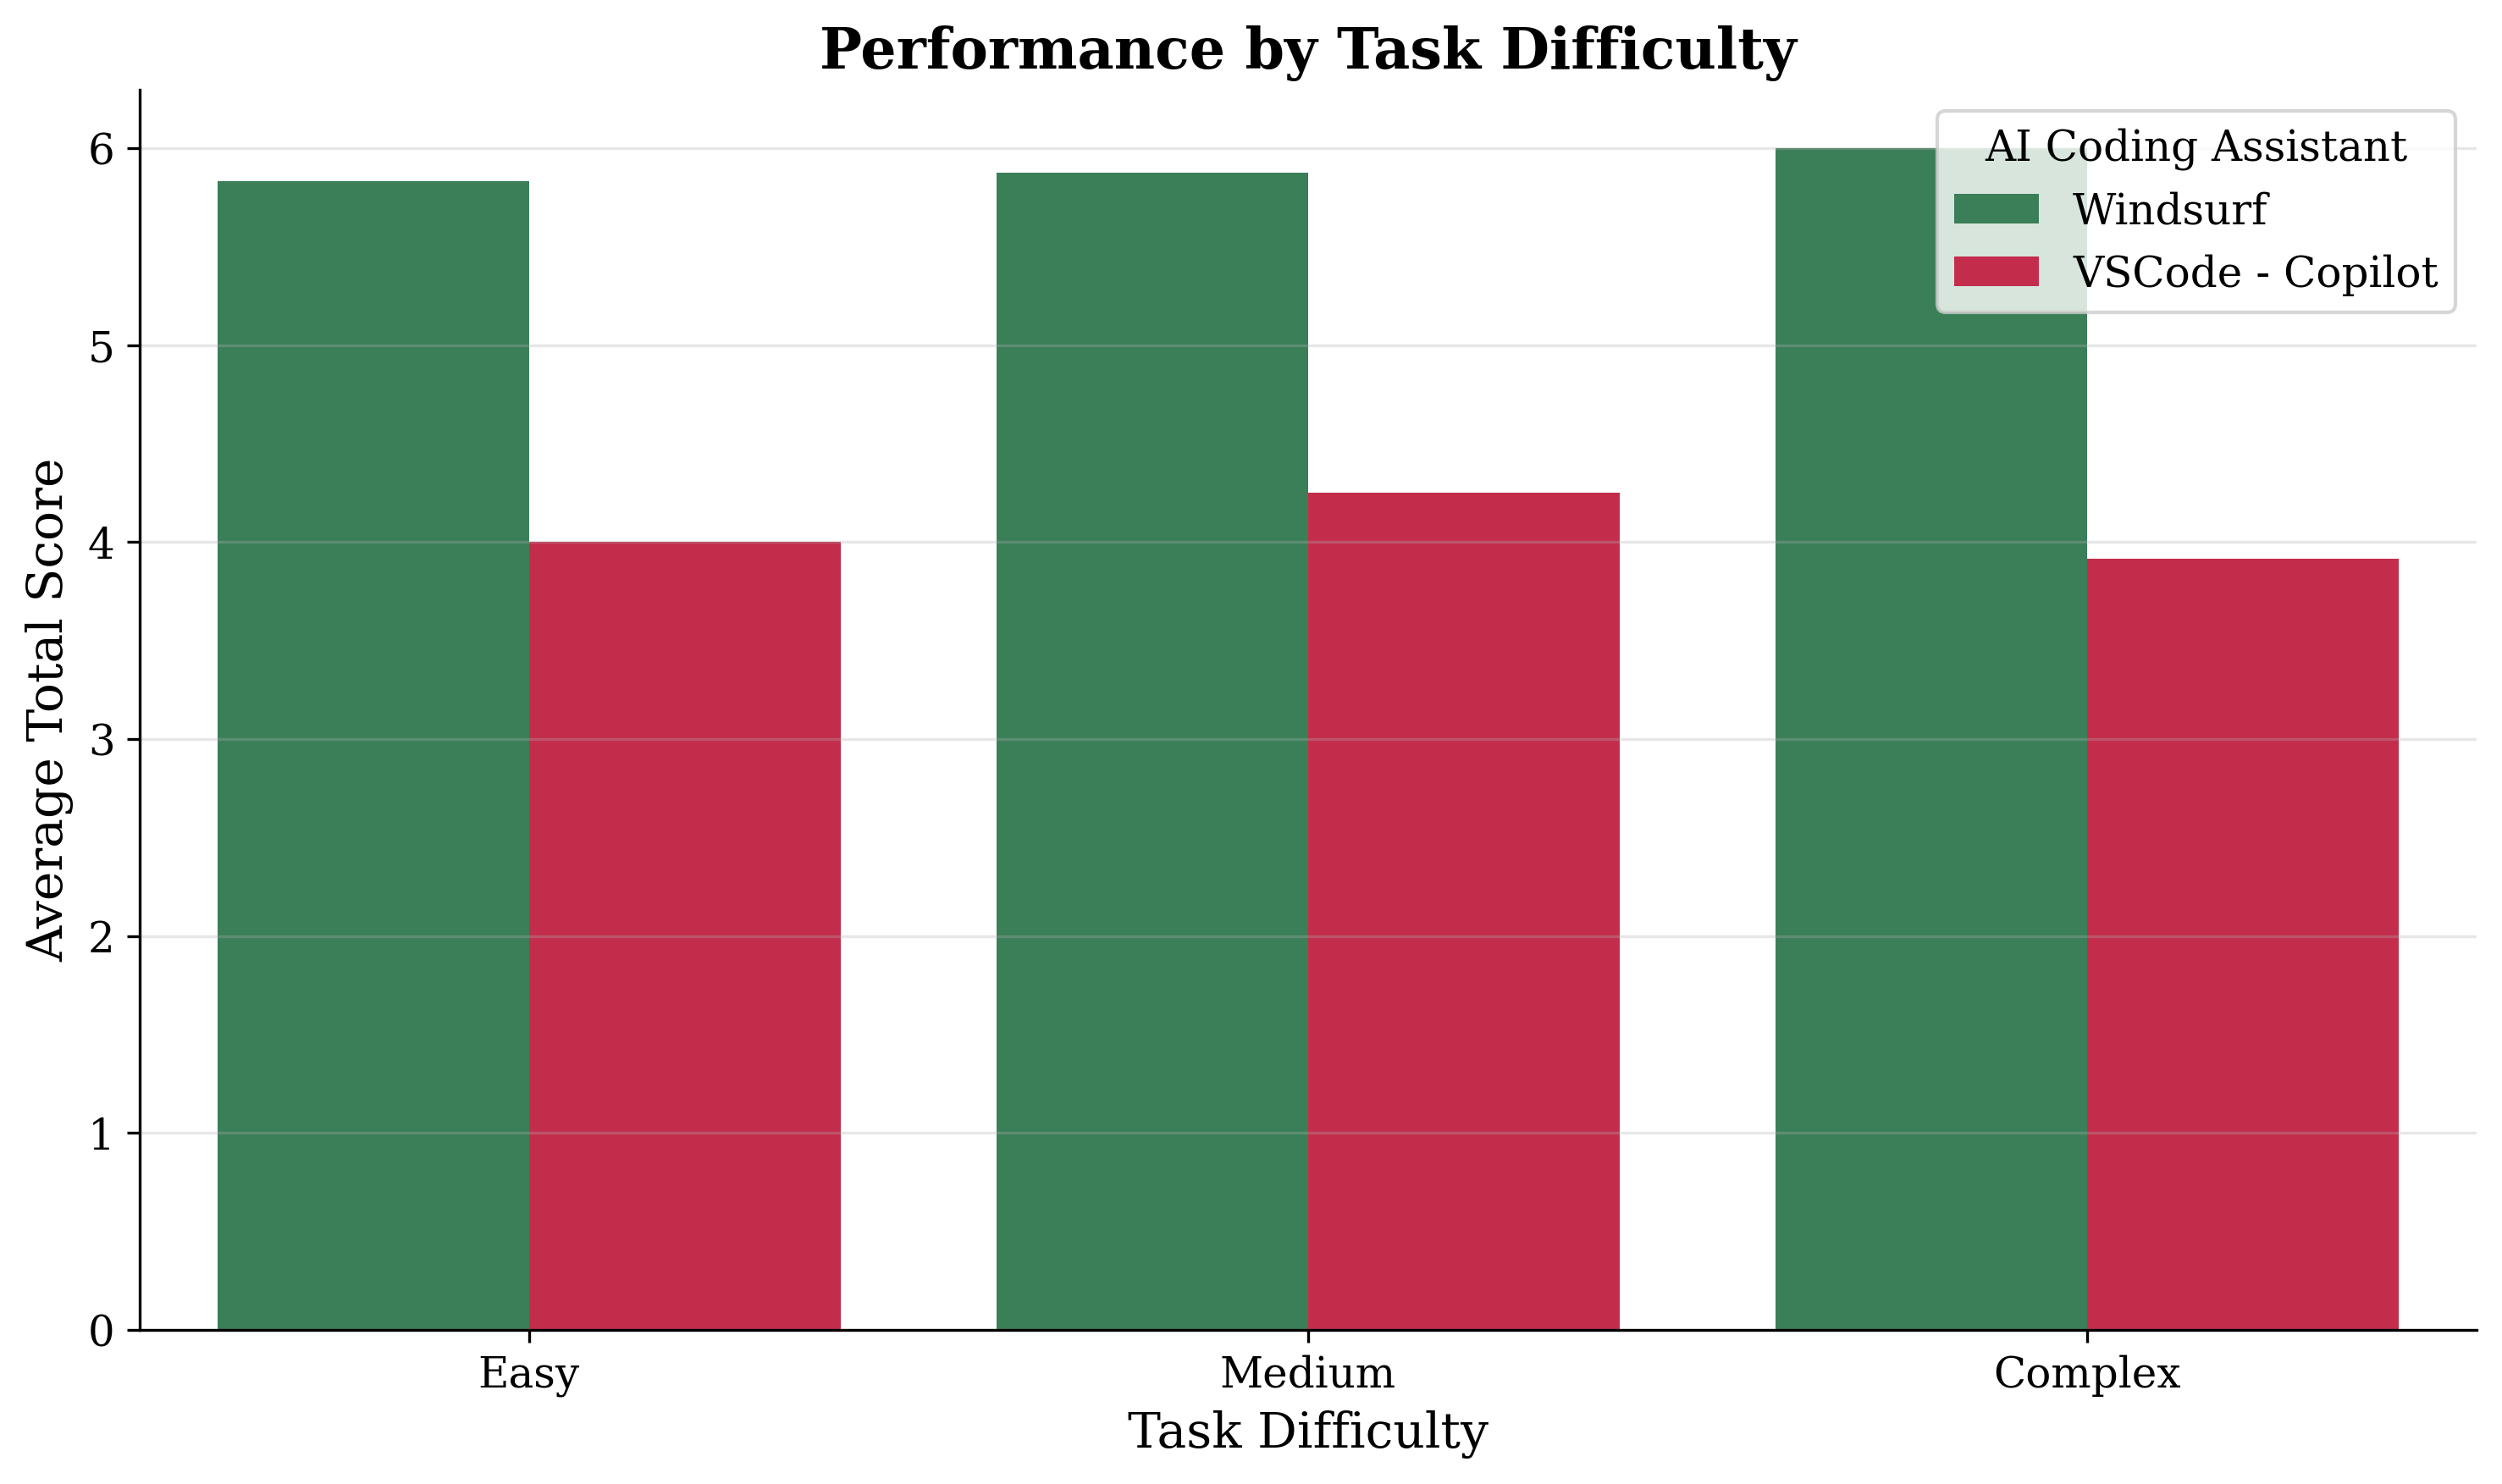
\includegraphics[width=1\linewidth]{images/3_difficulty_performance.png}
  \caption{Compared the performance by task difficulty of all executions of Windsurf Cascade and Github Copilot}
  \label{fig:performance-tasks}
\end{figure}

Figure \ref{fig:performance-tasks} shows the average score of the systems based on the three categories easy, medium and complex and compares the two systems with each other in these respects. In the easy category, Windsurf achieved an average score of 5.83 out of 6 points, in the medium category 5.88 out of 6 points and in the complex tasks the maximum score of 6 out of 6 points. Github Copilot achieved an average score of 4 out of 6 points in the easy category, 4.25 out of 6 points in the medium category prompts, and an average score of 3.92 out of 6 points in the complex tasks.


\begin{figure}[htbp]
  \centering
  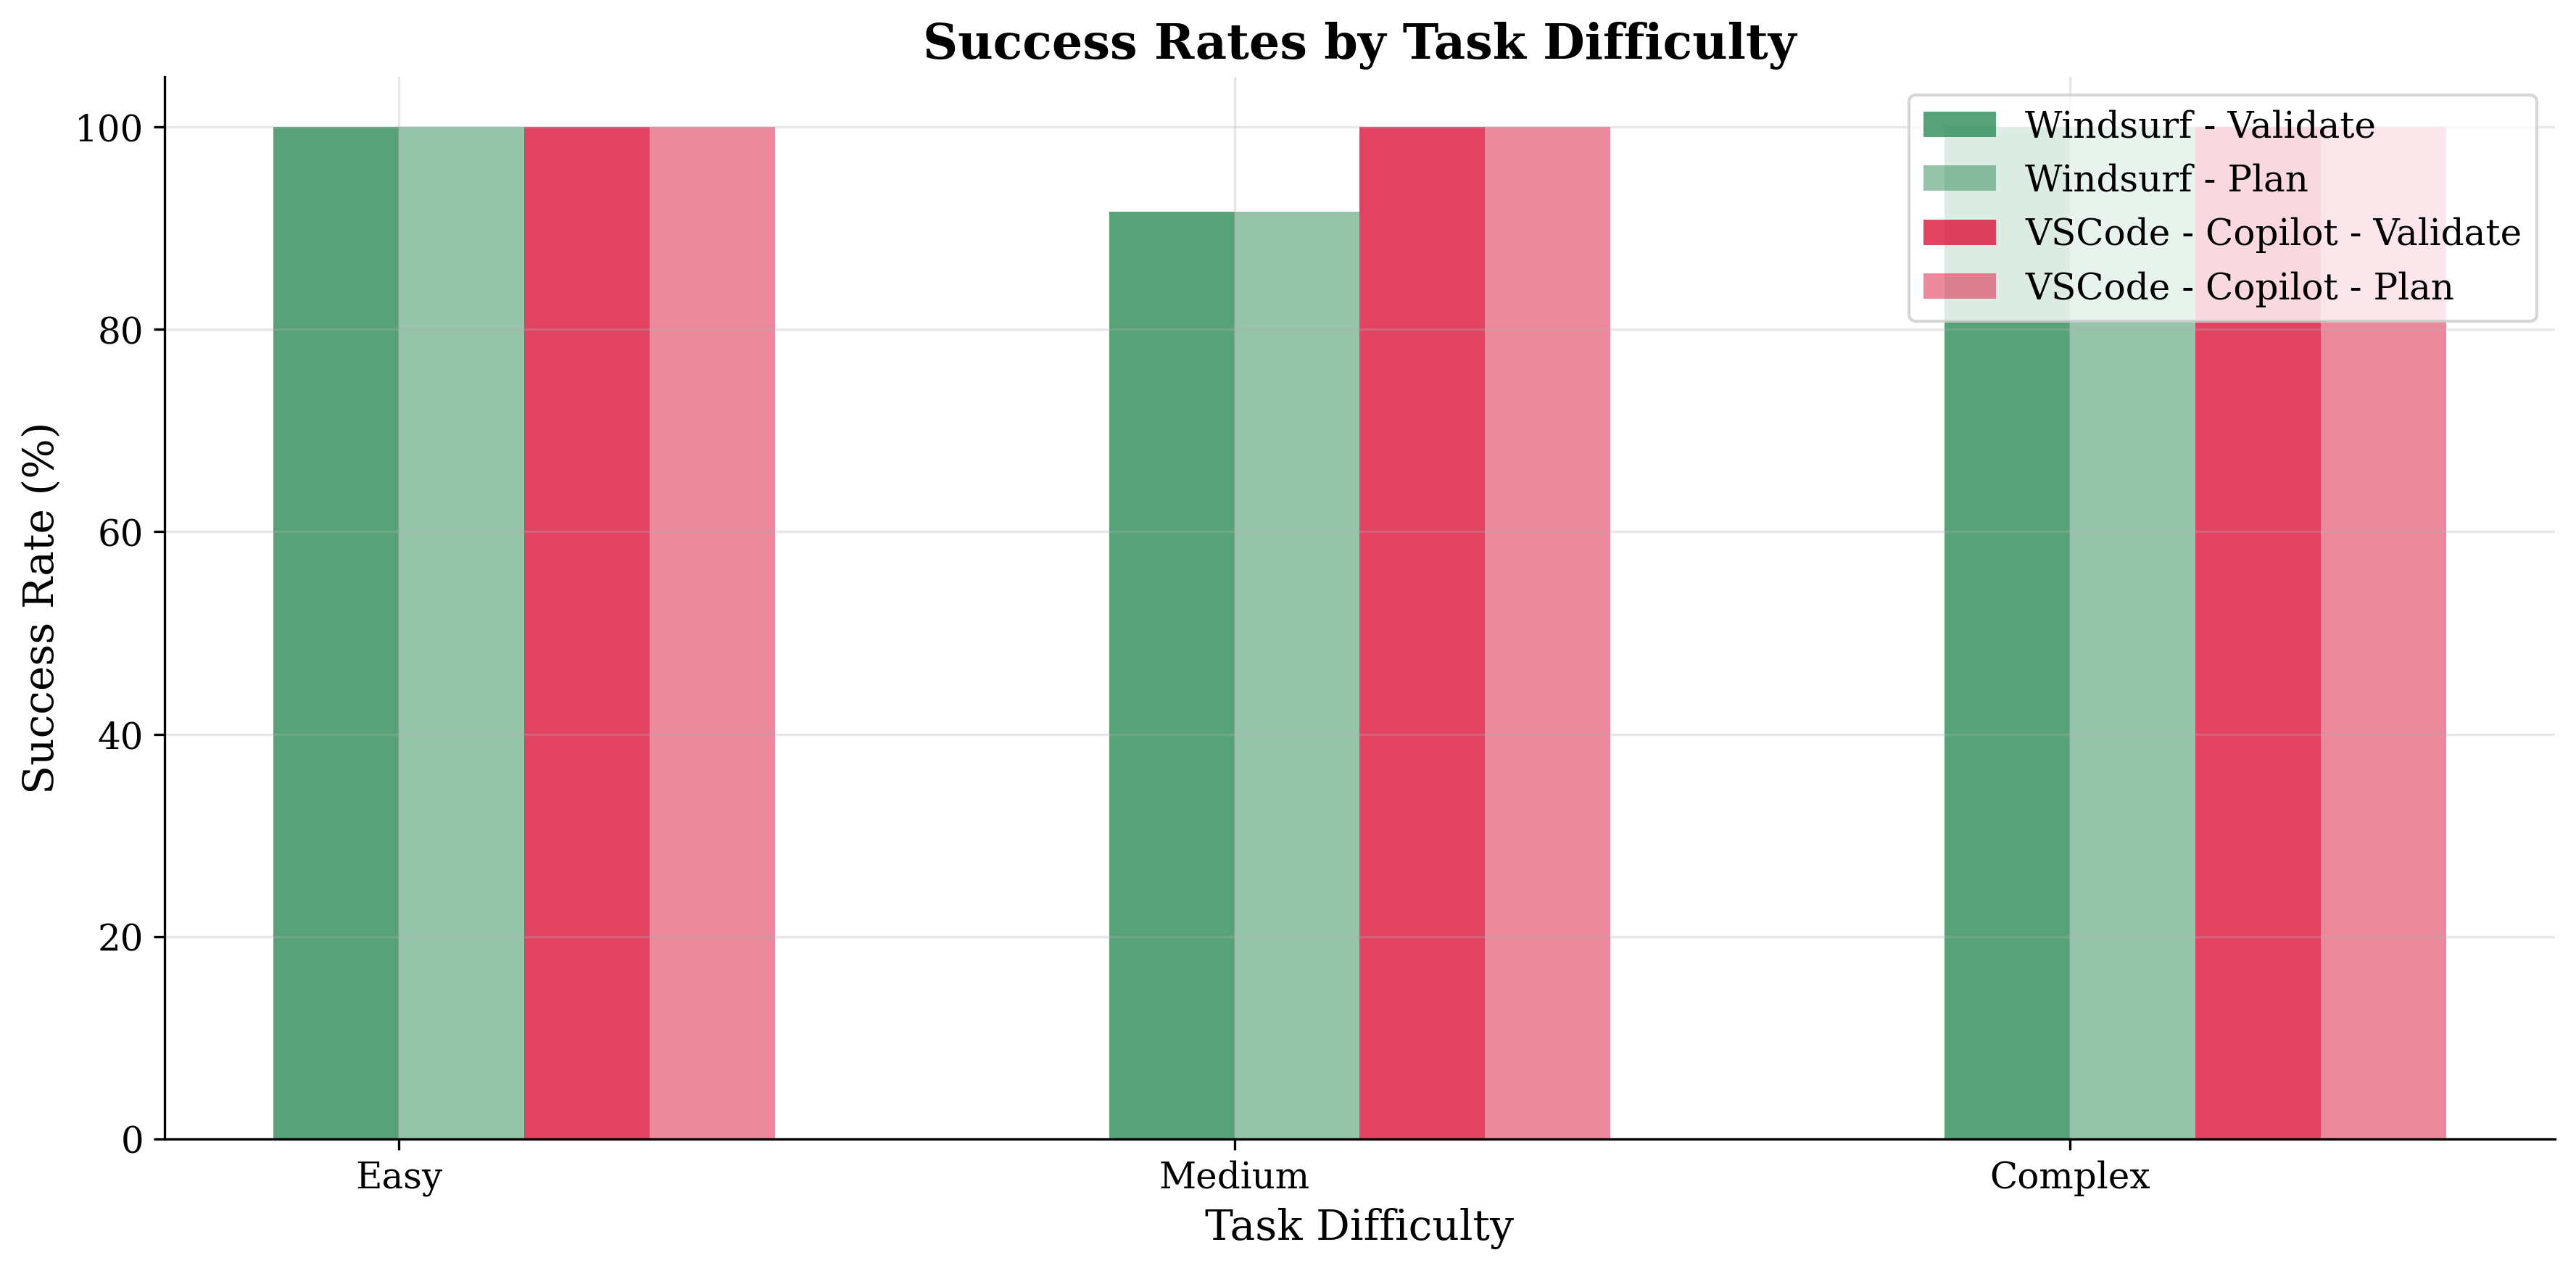
\includegraphics[width=1\linewidth]{images/7_success_by_difficulty.png}
  \caption{Compared the success of the validate and plan operation across all executions of Windsurf Cascade and Github Copilot}
  \label{fig:operation-success}
\end{figure}

Figure \ref{fig:operation-success} shows the success rates of the evaluation commands ''terraform validate'' and ''terraform plan'' executed after each evaluation of a prompt. Overall, Windsurfe Cascade achieved a success rate of 97\%, while Github copilot achieved a success rate of 100\% over both operations and all executions.
